\documentclass[conference, a4paper]{IEEEtran}
\IEEEoverridecommandlockouts

\usepackage{cite}
\usepackage{amsmath,amssymb,amsfonts}
\usepackage{algorithmic}
\usepackage{graphicx}
\usepackage{textcomp}
\usepackage{xcolor}
\usepackage{float}
\usepackage{subcaption}
\usepackage{booktabs}

\graphicspath{{../../../graphics}{../../../graphics/planar_dielectric_waveguide}{../../../graphics/rectangular_dielectric_waveguide}{../../../graphics/comsol_individual_waveguide}{../../../graphics/comsol_coupled_waveguide}}

\def\BibTeX{{\rm B\kern-.05em{\sc i\kern-.025em b}\kern-.08em
    T\kern-.1667em\lower.7ex\hbox{E}\kern-.125emX}}
\begin{document}

\title{Coupled Mode Theory and 50/50 Splitter}

\author{\IEEEauthorblockN{Eduardo A. V. Souza, RA: 250950}
\IEEEauthorblockA{\textit{"Gleb Wataghin" Institute of Physics} \\
\textit{UNICAMP}\\
Campinas, Brazil}
\and
\IEEEauthorblockN{Ivan Prearo (RA 237215)}
\IEEEauthorblockA{\textit{"Gleb Wataghin" Institute of Physics} \\
\textit{UNICAMP}\\
Campinas, Brazil}}

\maketitle

\begin{abstract}
    In this work, we aimed to design a 50/50 splitter made a two-waveguide coupled system. First, we started with a pre-analysis with COMSOL to optimize the material of the waveguides, their width and thickness, alongside with a resonable gap to obtain a short in length splitter. Then, we followed to the theoretical modeling of the problem based on Coupled Mode Theory, ranging from the derivation of the coupling constant formula, the coupled mode equations, and a numerical method to calculate the coupling rate. At the end, we analysed two cases of beamplitter, the first with identical waveguides, and the second with one waveguide with doubled dimensions. We found that the second case is better to obtain a more compact splitter.
\end{abstract}

\begin{IEEEkeywords}
    Waveguides, Coupled Mode Theory, Beamsplittersnsing.
\end{IEEEkeywords}

\section{Introduction}
\label{sec:intro}

In this section, we aim to describe the investigation to choose the material and the geometrical parameters of the waveguides belonging the coupled system. In the first place, we considered $SiO_2$, $TiO_2$, $Si_3N_4$, and $Ag_3AsS_3$ as the possible materials due to their renowed applications in photonic integrated circuits (PIC). Fig. \ref{fig:intro_dispersion} displays the dispersion of each one of these materials. As it is evident, $Ag_3AsS_3$ has the greatest values of refracive index (RI) and $SiO_2$ has the lowest, while $TiO_2$ and $Si_3N_4$ are intermediate cases. 

\begin{figure}[H]
    \centering
    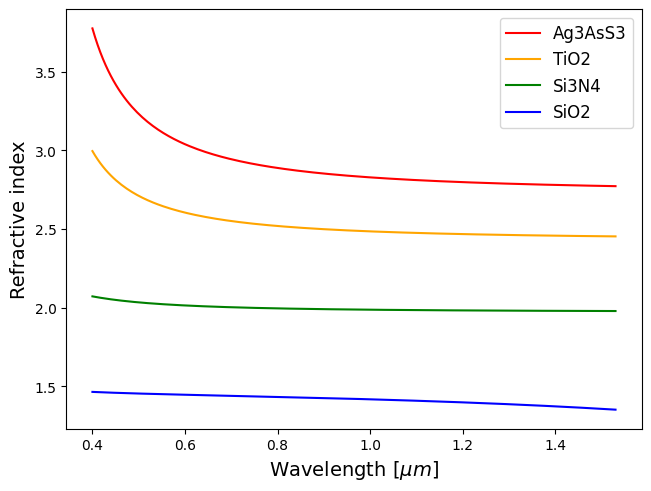
\includegraphics[scale=0.4]{dispersion_relation.png}
    \caption{Dispersion relation for the $SiO_2$, $TiO_2$, $Si_3N_4$, and $Ag_3AsS_3$.}
    \label{fig:intro_dispersion}
\end{figure}

Motivated by the common use of $SiO_2$ and $TiO_2$ in waveguides, and the info they present distinctive dispersion relations, $TiO_2$ presenting the highest values, we will focus on these materials as the candidates for the beam splitter. So, their dispersion relations are described by Eq. \eqref{eq:intro_dispersion}.

\begin{subequations}
    \begin{align}
        n_{SiO_2} &= 
        \sqrt{\begin{aligned}[t]
            &1 + \frac{0.6961663 \lambda^2}{\lambda^2 - 0.0684043^2} 
            + \frac{0.4079426 \lambda^2}{\lambda^2 - 0.1162414^2} \\
            &+ \frac{0.8974794 \lambda^2}{\lambda^2 - 9.896161}
        \end{aligned}}
    \end{align}
    \begin{align}
        n_{TiO_2} &= \sqrt{5.913 + \frac{0.2441}{\lambda^2 - 0.0803}}
    \end{align}
    \label{eq:intro_dispersion}
\end{subequations}

To understand the number of modes in a waveguide, we plotted the characteristic equations for $SiO_2$ for the infinite dielectric slab case, which has a easier mathematical description. The generic characteristic equation is described by Eq. \eqref{eq:intro_equation} where $d$ is the thickness of the slab, and the plot of the functions describing this equation, $f_1$ and $f_2$, are plotted in Fig. \ref{fig:intro_equation}.

\begin{equation}
    \begin{split}
        f_1(\sin(\theta)) 
        &\equiv \tan\left[ \pi \left(\frac{\sin(\theta) d}{\lambda} - \frac{m}{2}\right) \right] \\
        &= \sqrt{\frac{\sin^2(\overline{\theta}_c)}{\sin^2(\theta)} - 1} \equiv f_2(\sin(\theta))
    \end{split}
    \label{eq:intro_equation}
\end{equation}

\begin{figure}[H]
    \centering
    \centering
    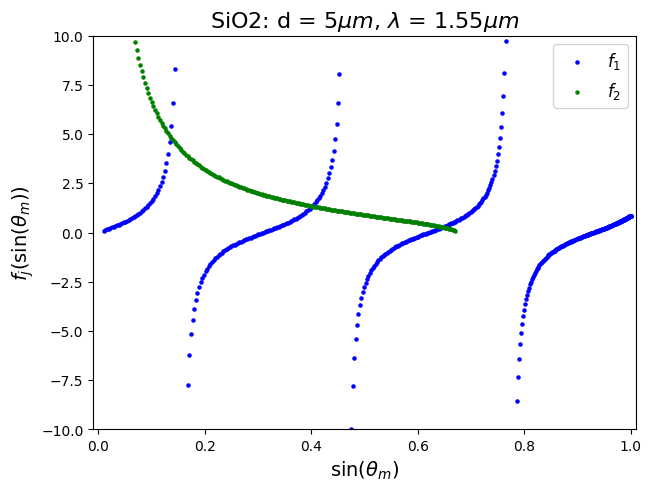
\includegraphics[scale=0.4]{modes_SiO2_d5um_wv1.55um.png}
    \caption{$SiO_2$.}
    \caption{Plot of the characteristic equations for the $SiO_2$ and $TiO_2$ infinite slab case.}
    \label{fig:intro_equation}
\end{figure}

From Fig. \ref{fig:intro_equation} it is evident $f_1$ and $f_2$ intersect at three points, that is, this waveguide presents only three modes. As we increase the thickness of the slab, we make room for more modes to appear. As the next step, we plotted the characteristic functions for the rectangular dielectric case for $SiO_2$ and $TiO_2$, considering the approximation $E(x, y) = X(x) Y(y)$. Considering these components independent, we can solve the characteristic equation for x and y dimensions separately, find $\theta_{mx}$ and $\theta_{my}$, and latter on combine into the solution described by Eq. \eqref{eq:intro_rectangle} where $k_{j} = n_1 k_0 \sin(\theta_{m_j}), \ \forall j \in\{1, 2\}$.

\begin{equation}
    \beta_{m_x, m_y} = \sqrt{(n_1 k_0)^2 - k_x^2 - k_y^2}
    \label{eq:intro_rectangle}
\end{equation}

With the results above, we could note the waveguide made of $SiO_2$ presented a smaller number of modes when compared to the $TiO_2$ case. Since in this work we are concerned with a waveguide with a few guided modes only, we decided to explore the coupled system made of $SiO_2$ cores and the geometrical parameters $t_{core,j} = 2\mu m$, (i) $w_{core, j} = 6 \mu m$, and (ii) $w_{core, 2} = 2 w_{core, 1} = 6\mu m$ and $t_{core, j} = 2\mu m$. Another observation, is that we are considering the two cores for the coupled systems to be aligned at the center of the cartesian coordiniate system, in a sense the gap in the y-direction is $d_y = 0$, otherwise it would distort the overlapping region and would not give much different information. Thus, we can name the gap in the x-direction simply $d$.

\section{Theoretical development}
\label{sec:theory}

\subsection{Coupling coefficient}
\label{subsec:theory_coefficient}

\subsection{Coupled equations}
\label{subsec:theory_equations}

\section{50/50 splitter}
\label{sec:splitter}

In this section, we aim to effectively model the 50/50 splitter describe at the end of Sec. \ref{sec:intro} with COMSOL with the cores made by $SiO_2$ and the cladding made of air with the following geometrical parameters $t_{clad} = 15\mu m$ and $w_{clad} = 30\mu m$. So, we discuss the case of two identical cores with $t_{core} = 2\mu m$ and $w_{core} = 6\mu mu$ in Subsec. \ref{subsec:splitter_identical} and in Subsec. \ref{subsec:splitter_doubled} we analyse what changes if we let the first core to have width $w_{core, 1} = w_{core, 2}/2 = 3\mu m$, that is, core 2 presents the double width of core 1.
    
\subsection{Identical cores}
\label{subsec:splitter_identical}

For this subsection and the following, it is important to note we are considering $1.55\mu m$ as the reference input wavelength due its huge applicability in telecommunication and just the first even and odd supermodes. Also, we are separating the even supermodes from the odd ones based on the arrow surface plot of $\mathbf{E}_x$ vs. $\mathbf{E}_y$ onto the surface plot of $\| \mathbf{E} \|$ as indicated in Fig. \ref{fig:splitter_identical_parity}. The even modes present arrows in the same direction for both cores, and the odd present arrows in the opposite direction.

\begin{figure}[H]
    \centering
    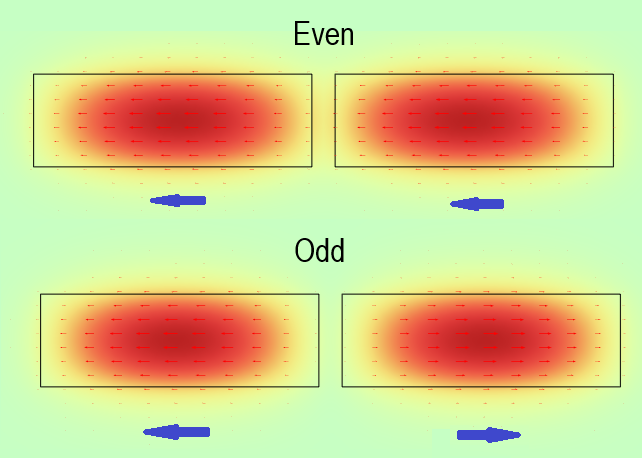
\includegraphics[scale=0.4]{even_odd_supermodes.png}
    \caption{Distinction between even and odd supermodes $SiO_2$ core with $w_{core, j} = 6\mu m$ and $t_{core, j} = 2\mu m$, and the gap between cores given by $d = 0.5\mu m$.}
    \label{fig:splitter_identical_parity}
\end{figure} 

We varied the gap between the cores and decided to use $d = 0.5mu m$ due its considerable overlapping region and because lower gaps might be difficult to frabricate with techniques such as photolitography.

% Place here the value for the coupling constant...

Aiming to explore the sensitivity of this splitter with the wavelength, we repeated the simulation for the range $\lambda \in [1.40 \mu m, 1.70 \mu m]$ and obtained from COMSOL the effective refractive index $n_{eff}$ for each supermode. Using $\beta = k_0 n_{eff}$, we could obtain the propagation constant for each supermode mode as well.

Once we now the order of the even and odd supermodes for a given wavelength, we can compute the coupling length $L_c$, the length needed for the light being initally guided through the first core to be entirely coulpled into the second core. To do so, we used Eq. \eqref{eq:splitter_identical_lc}, where $\Delta \beta \equiv \beta_{even} - \beta_{odd}$. These values are place in Tab. \ref{tab:splitter_identical_lc}, which also displays the coupling efficiency $\eta$ from the first core into the second one considering a intercation length of $L_{int} = 484.4\mu m$.

\begin{equation}
    L_c = \frac{\pi}{\Delta \beta}
    \label{eq:splitter_identical_lc}
\end{equation}

\begin{table}[H]
    \centering
    \begin{tabular}{ccc}
        \toprule
        $\lambda [\mu m]$ & $L_c$ & $\eta[\%]$ \\
        \midrule
        1.40 & 1400.0 & 34.6 \\
        1.45 & 1450.0 & 33.4 \\
        1.50 & 1071.4 & 45.2 \\
        1.55 & 968.7 & 50.0 \\
        1.60 & 888.9 & 54.5 \\
        1.65 & 750.0 & 64.59 \\
        1.70 & 653.8 & 74.09 \\    
        \bottomrule
    \end{tabular}
    \caption{Coupling length and coupling efficiency coefficient for the first supermode making $L_{int} = 484.4\mu m$ varying the input wavelength for the identical cores.}
    \label{tab:splitter_identical_lc}
\end{table}

As you can see from the table above, the operational range of this 50/50 beamplitter is short, it can operate within a 5\% margin of $\eta$ in the range $\lambda \in [1.50\mu m, 1.60\mu m]$, a span of $100nm$ only. Also, if we cconsider a fabrication error in the interation length of 10\%, we would have a coupling interval in $1.55 \mu m$ of $\eta \in [45\%, 55\%]$.  

\subsection{First core with half width}
\label{subsec:splitter_doubled}

For the case of the first core to present half the widht of the second, we repeated the same analysis of Subsec. \ref{subsec:splitter_identical}. 

% Place here the values for the coupling coefficient...

The wavelength sensitivity is analysed in Tab. \ref{tab:splitter_doubled_lc}. As you can see, the $\eta$ vary much less with the wavelength than the previous case. For the range $\lambda \in [1.40 \mu m, 1.70 \mu m]$, a span of $300nm$, $\eta$ has a margin less than 2\%. Thus, if we accept a margin of 5\%, we could extend even further the wavelength range. Again, if we consider a fabrication error in the interaction length of 10\% for $1.55\mu m$ input wavelength, we would obtain a efficiency interval of $[45\%, 55\%]$. In this case, the interaction length error would contribute more to the deviation of the 50/50 coupling when compared to the wavelength variation.

\begin{table}[H]
    \centering
    \begin{tabular}{ccc}
        \toprule
        $\lambda [\mu m]$ & $L_c$ & $\eta[\%]$ \\
        \midrule
        1.40 & 179.5 & 49.1 \\
        1.45 & 176.8 & 49.8 \\
        1.50 & 174.4 & 50.5 \\
        1.55 & 176.1 & 50.0 \\
        1.60 & 170.2 & 51.8 \\
        1.65 & 175.5 & 50.2 \\
        1.70 & 177.1 & 49.7 \\    
        \bottomrule
    \end{tabular}
    \caption{Coupling length and coupling efficiency coefficient for the first supermode making $L_{int} = 88.1\mu m$ varying the input wavelength for different size cores.}
    \label{tab:splitter_doubled_lc}
\end{table}

\section{Conclusion}
\label{sec:conclusion}

In summary, we began our study with a investigation of the material of cores for the coupled system, their geometry and the gap distance between them. In sequence, we derived the coupling coefficient form and the coupled mode equations, followed by the discussion of a numerical method to compute the coupling rate. At last, we projected two cases of a 50/50 beamplitter varying the geometry of the cores, and analyse their sensitivity with the wavelength and the length interaction error.

% \bibliographystyle{IEEEtran}
% \bibliography{References}


\end{document}
